%%%%%%%%%%%%%%%%%%%%%%%%%%%%%%%%%%%%%%%%%
% Stylish Article
% LaTeX Template
% Version 2.1 (1/10/15)
%
% This template has been downloaded from:
% http://www.LaTeXTemplates.com
%
% Original author:
% Mathias Legrand (legrand.mathias@gmail.com) 
% With extensive modifications by:
% Vel (vel@latextemplates.com)
%
% License:
% CC BY-NC-SA 3.0 (http://creativecommons.org/licenses/by-nc-sa/3.0/)
%
%%%%%%%%%%%%%%%%%%%%%%%%%%%%%%%%%%%%%%%%%

%----------------------------------------------------------------------------------------
%	PACKAGES AND OTHER DOCUMENT CONFIGURATIONS
%----------------------------------------------------------------------------------------

\documentclass[fleqn,10pt]{SelfArx} % Document font size and equations flushed left

\usepackage[english]{babel} % Specify a different language here - english by default
\usepackage{subcaption}

\usepackage{lipsum} % Required to insert dummy text. To be removed otherwise
\usepackage{listings}

%----------------------------------------------------------------------------------------
%	COLUMNS
%----------------------------------------------------------------------------------------

\setlength{\columnsep}{0.55cm} % Distance between the two columns of text
\setlength{\fboxrule}{0.75pt} % Width of the border around the abstract

%----------------------------------------------------------------------------------------
%	COLORS
%----------------------------------------------------------------------------------------

\definecolor{color1}{RGB}{0,0,90} % Color of the article title and sections
\definecolor{color2}{RGB}{0,20,20} % Color of the boxes behind the abstract and headings

%----------------------------------------------------------------------------------------
%	HYPERLINKS
%----------------------------------------------------------------------------------------

\usepackage{hyperref} % Required for hyperlinks
\hypersetup{hidelinks,colorlinks,breaklinks=true,urlcolor=color2,citecolor=color1,linkcolor=color1,bookmarksopen=false,pdftitle={Title},pdfauthor={Author}}

%----------------------------------------------------------------------------------------
%	ARTICLE INFORMATION
%----------------------------------------------------------------------------------------

\JournalInfo{Development Research Group, The World Bank} % Journal information
\Archive{February 2017} % Additional notes (e.g. copyright, DOI, review/research article)

\PaperTitle{Using Convolutional Neural Networks for Land Use Detection on Satellite Imagery} % Article title

\Authors{LA\textsuperscript{1}\textsuperscript{2}, KS\textsuperscript{2}} % Authors
\affiliation{\textsuperscript{1}\textit{UB}}
\affiliation{\textsuperscript{2}\textit{WB}}

\Keywords{Machine Learning -- Computer Vision --- Remote Sensing --- Convolutional Neural Network} % Keywords - if you don't want any simply remove all the text between the curly brackets
\newcommand{\keywordname}{Keywords} % Defines the keywords heading name

%----------------------------------------------------------------------------------------
%	ABSTRACT
%----------------------------------------------------------------------------------------

\Abstract{Convolutional Neural Networks (CNNs) are one of the machine learning methods used for pixel-wise classification of image data. Based on the SegNet framework, a data pipeline was developed to classify satellite images using Geographic Information System (GIS) data that includes parsing the GIS data, requesting the necessary satellite imagery, creating the training data, traning the network based on Graphics Processing Units (GPUs) and applying the classifier. This report gives a short technical overview on the pipeline software.
}

%----------------------------------------------------------------------------------------

\begin{document}

\flushbottom % Makes all text pages the same height

\maketitle % Print the title and abstract box

\tableofcontents % Print the contents section

\thispagestyle{empty} % Removes page numbering from the first page

%----------------------------------------------------------------------------------------
%	ARTICLE CONTENTS
%----------------------------------------------------------------------------------------

\section{Introduction} % The \section*{} command stops section numbering
Convolutional neural networks (CNNs) have recently seen great interest, including from the areas of particle physics  -- especially in neutrino physics \cite{Barnard:2016qma}\cite{Aurisano:2016jvx}\cite{Racah:2016gnm}\cite{Acciarri:2016ryt} -- and remote sensing \cite{xu2008cnn}\cite{hu2015transferring}. Pixel-wise semantic labelling is used for segmentation of images and is efficiently performed by CNNs \cite{BadrinarayananK15}. 

SegNet is a framework developed by Bandrinarayanan et al. based on the Caffe deep learning architecture \cite{jia2014caffe} that uses CNNs for pixel-wise semantic labelling \cite{BadrinarayananK15}. By embedding SegNet to a Geographic Information System (GIS) data pipeline on an early stage, the usage of CNNs for satellite imagery should be possible for research \& development purposes.

%------------------------------------------------

\section{Pipeline}
The purpose of the data pipeline software -- called CV4AG (Convolution for Agriculture) -- is to train CNNs and classify satellite images by GIS input data. The software has been developed as an open source project (\url{https://github.com/worldbank/cv4ag/}) working within the Python and Caffe SegNet environments. The pipeline consists of different stages:
\begin{itemize}[noitemsep]
\item  parsing, 
\item getting satellite data,
\item  overlaying images, 
\item training the CNN and 
\item applying the machine learning algorithm.
\end{itemize}
 These can be called all together with the command
\begin{lstlisting}[language=bash]
  $ python cv4ag.py -i $Inputfile \
	all $MapboxToken
\end{lstlisting}

 or separately, as indicated in the subsections.

\begin{figure*}[ht]\centering % Using \begin{figure*} makes the figure take up the entire width of the page
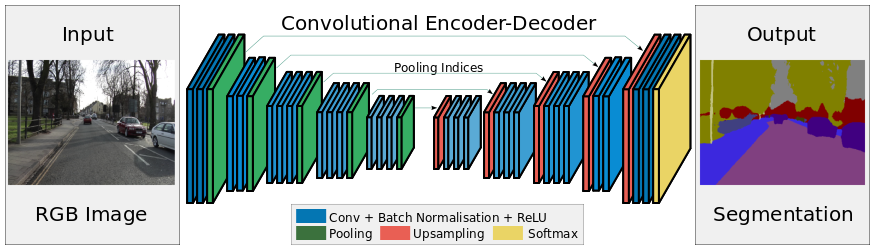
\includegraphics[width=\linewidth]{segnet1.png}
\caption{Architecture of a SegNet Convolutional Neural Network. \textit{Source:} \cite{BadrinarayananK15}.}
\label{fig:view}
\end{figure*}
\subsection{Parsing}
\begin{lstlisting}[language=bash]
  $ python cv4ag.py -i $Inputfile parse
\end{lstlisting}
or
\begin{lstlisting}[language=bash]
  $ python cv4ag.py -s OSM_Query.py\
	--arg1 GB parse
\end{lstlisting}
The parser can acquire date from two sources: Either a GIS vector file, or by using OpenStreetMap (OSM, \url{http://www.openstreetmap.org}) data.
The GIS input file will form the training data and should be in vector format. It is converted into GeoJSON format using the \textsc{GDAL} library.
Alternatively, a script for getting OSM data can be executed, with the country to extract features from given as an argument in form of the 2-letter ISO country code.

The parser extracts frequency statistics of the most frequent classes that later will be used to determine the categorisation classes.
Vectorisation for non-vector GIS input data is planned to be implemented in order to enable classification of raster GIS source data.

\subsection{Get satellite imagery}
\begin{lstlisting}[language=bash]
  $ python cv4ag.py -i $Inputfile \
	satellite $MapboxToken
\end{lstlisting}
According to the position of the polygons of the input file, satellite images are downloaded via Mapbox API (\url{http://www.mapbox.com}). In order to do so, coordinates are converted into WGS-1984 format. The zoom levels can be defined, with the resolution given in table~\ref{tab:label}.
\begin{table}[hbt]
\caption{Zoom levels}
\centering
\begin{tabular}{lllll}
\toprule
Zoom level $\|$ Latitude & $0^\mathrm{o}$ & $15^\mathrm{o}$ & $30^\mathrm{o}$ & $45^\mathrm{o}$ \\
\midrule
\textbf{15}&$4.78\mathrm{m}$&$ 4.61\mathrm{m}$&$ 4.14\mathrm{m}$&$ 3.38\mathrm{m}$\\
\textbf{16}&$2.39\mathrm{m}$&$ 2.31\mathrm{m}$&$ 2.07\mathrm{m}$&$ 1.69\mathrm{m}$\\
\textbf{17}&$1.19\mathrm{m}$&$ 1.15\mathrm{m}$&$ 1.03\mathrm{m}$&$ 0.84\mathrm{m}$\\
\textbf{18}&$0.60 \mathrm{m}$&$ 0.58\mathrm{m}$&$0.52\mathrm{m}$&$0.42\mathrm{m}$\\
\textbf{19}&$0.30\mathrm{m}$&$ 0.29\mathrm{m}$&$ 0.26\mathrm{m}$&$ 0.21\mathrm{m}$\\
\textbf{20}&$0.15\mathrm{m}$&$ 0.14\mathrm{m}$&$ 0.13\mathrm{m}$&$ 0.11\mathrm{m}$\\
\bottomrule
\end{tabular}
\label{tab:label}
\end{table}
Satellite data are either chosen randomly within the boundery box of the GIS data, or are selected as the centre points of the polygons. 


\subsection{Overlay images}
\begin{lstlisting}[language=bash]
  $ python cv4ag.py -i $Inputfile overlay
\end{lstlisting}
The overlay module creates the class label images. It extracts the single features from the GIS file, determines the location of a GIS file polygon on the satellite image and finally creates a PNG file for each satellite image with each of the greyscale values corresponding to a specific class. Check images -- such as shown in figure~\ref{fig:results} -- are created in order to detect shifts and inaccuracies in the GIS data or in coordinate mapping. The module uses parallel multi-core processing.
\begin{figure}[ht]\centering
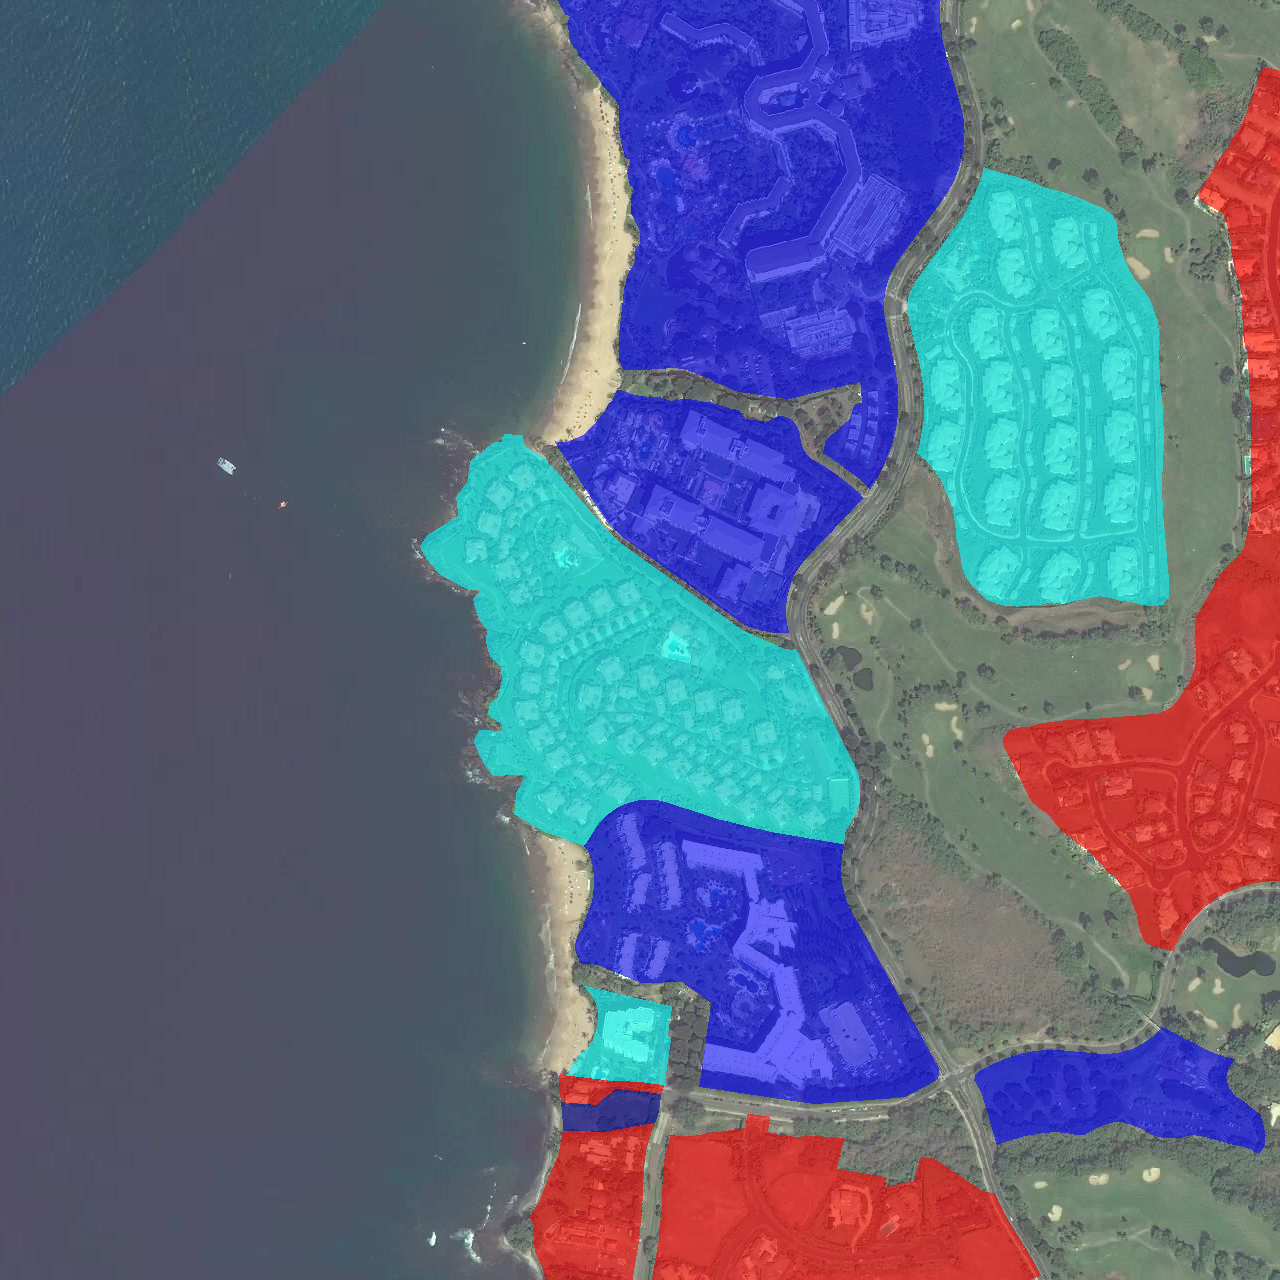
\includegraphics[width=\linewidth]{hawaii}
\caption{Check image for OSM land use input data (satellite data overlaid with class labels) from Hawaii, United States.}
\label{fig:results}
\end{figure}

\subsection{Training}
\begin{lstlisting}[language=bash]
  $ python cv4ag.py -i $Inputfile train 
\end{lstlisting}
The training module trains the CNN applying Caffe SegNet. This includes extrating statistics, generating the model files and running a steeepest-gradient type training algorithm. Usually, Graphics Processing Units (GPUs) are used as they accelerate the training process significantly, but the trainig can be run in CPU mode. The created data from the previous stages can be split into test and training data, if necessary. Background, i.e. unlabelled pixels, can be treated as a class for its own or can be ignored. Training can take a high amount of time and its outcome depends not only on the amount of iterations, but also on the size of available GPU memory.
\begin{figure*}[ht]\centering % Using \begin{figure*} makes the figure take up the entire width of the page
\begin{subfigure}{.33\textwidth}
  \centering
  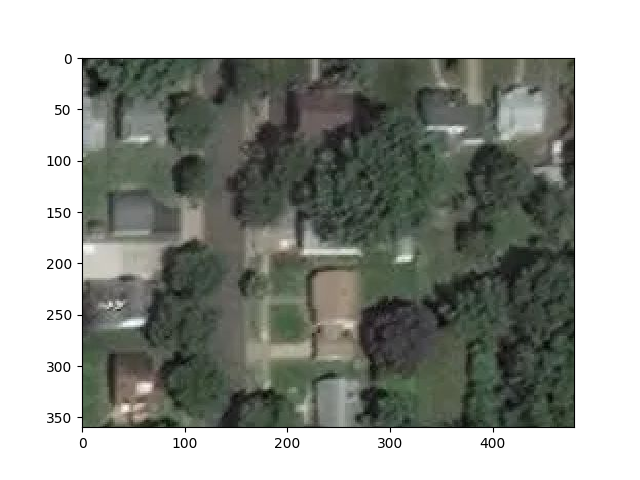
\includegraphics[width= \linewidth]{minnesota1.png}
  \caption{Satellite image.}
\end{subfigure}%
\begin{subfigure}{.33\textwidth}
  \centering
  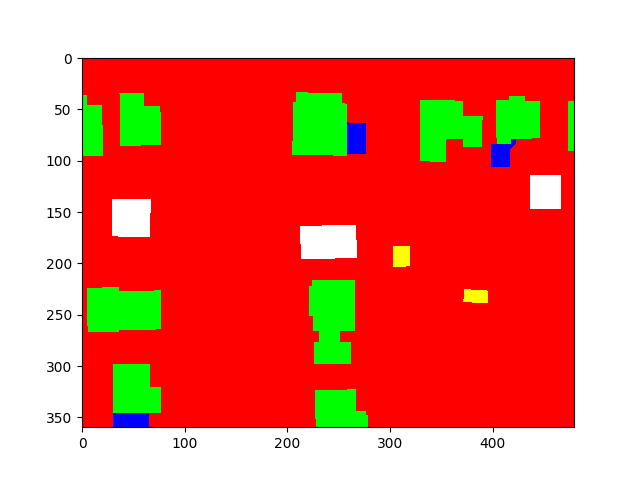
\includegraphics[width= \linewidth]{minnesota2.png}
  \caption{Labelled trainig image.}
\end{subfigure}%
\begin{subfigure}{.33\textwidth}
  \centering
  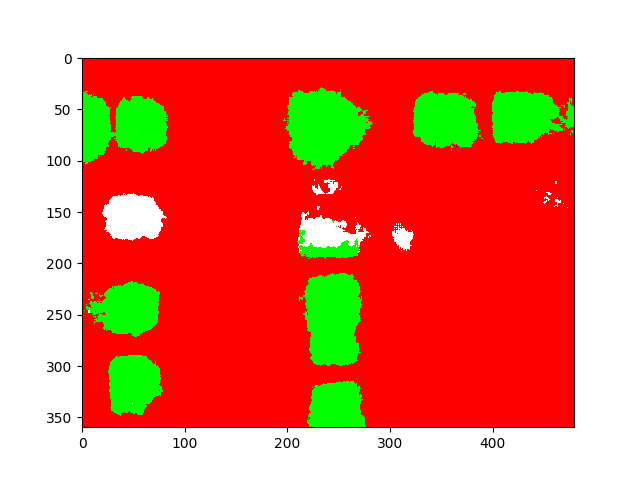
\includegraphics[width= \linewidth]{minnesota3.png}
  \caption{Pixel-wise classified image.}
\end{subfigure}
\caption{Classification of data based on Minnesota GIS data by the SegNet CNN. The image on the right is the output classified image by the Convolutional Neural Network. \textit{Green} denotes residential houses, \textit{grey} garages and \textit{red} background.}
\label{fig:ex}
\end{figure*}
\newpage
\subsection{Classification}
\begin{lstlisting}[language=bash]
  $ python cv4ag.py -i $Inputfile ml
\end{lstlisting}
The trained CNN is applied to test data within the classification module, i.e. the input test images get pixel-wise semantically labelled. The classification accuracy depends on the training quality. An example of classification is shown in figure~\ref{fig:ex}.



%------------------------------------------------


\section{Outlook}
A main task is to apply the pipeline to high-quality GIS data with full coverage of the respective bounderies. This also can be used to evaluate to which extend of accuracy and for which kind of satellite imagery the CNN pipeline is efficient. It is also intended to use high bandwith-satellite imagery beyond visible spectrum instead of RGB tiles for training. This is considered likely to improve performance of classification.
%------------------------------------------------


%----------------------------------------------------------------------------------------
%	REFERENCE LIST
%----------------------------------------------------------------------------------------
\phantomsection
\bibliographystyle{unsrt}
\bibliography{report_cv4ag}

%----------------------------------------------------------------------------------------
\newpage
\section*{Technical Documentation}
\addcontentsline{toc}{section}{Technical Documentation} % Adds this section to the table of contents
\subsection*{Output}
\addcontentsline{toc}{subsection}{Output} % Adds this section to the table of contents
The output tree structure that is created is
\begin{lstlisting}
outputFolder/inputFilename
 	 -sat (satellite data)
	 -train (training data)
	 -test (test data)
	 -check (check data)
	 -weights (CNN weights)
	 -out (CNN applied on images)
	 -models (CNN models)
	 -imgindex (index files)
	 -feature (feature layers) 
\end{lstlisting}
\subsection*{Usage} % The \section*{} command stops section numbering

\addcontentsline{toc}{subsection}{Usage} % Adds this section to the table of contents
\begin{lstlisting}
usage: cv4ag.py [-h] [-i FILE] [-s FILE]
		[-o PATH] [-c N] [-z N]
		[-x N] [-y N]
                [-d FILETYPE_CODE] [-n N]
		[--lonshift N.N]
		[--latshift N.N]
                [--shiftformat N]
		[--top N] [--key KEY] 
		[--epsg N] [--layer N]
                [--mode MODE] [--arg1 ARG1] 
		[--arg2 ARG2] [--arg3 ARG3]
                [--arg4 ARG4] 
		[--test | --no-test]
                [--background | --no-background] 
		[--random | --no-random]
                OPTION 
		[MAPBOX_TOKEN]

Machine Learning Framework for Agricultural Data.
positional arguments:
  OPTION        The modules to be loaded.
	        OPTIONs:
		all - all modules (except clear). 
		parse - input file parser. 
		satellite - get satellite data. 
		overlay - overlay classification with satellite data. 
		train - train. 
		ml - apply machine learning algorithm. 
		clear - clear generated data from previous run on input file
  MAPBOX_TOKEN  Mapbox token to download 
		satellite images.
\end{lstlisting}
\newpage\phantom{a}\newpage
\begin{lstlisting}

optional arguments:
  -h, --help        show this help message and exit
  -i FILE           Input file. Do not give if data 
			obtained by script.
  -s FILE           Script file to obtain data
  -o PATH           Output folder. Satellite data are 
			put in and read from
                    	PATH/sat/.
  -c N              Number of satellite images to download.
  -z N              Zoom level. Min=15, Max=19. See
                    	libs/satellite_resolutions.csv 
			for resolutions.
  -x N              Images have width N pixel.
  -y N              Images have height N pixel.
  -d FILETYPE_CODE  Specify file type. Will find to 
			detect filetype automatically. 
  -n N              Accuracy of neural net. 0: lowest. 
			3: highest.
  --lonshift N.N    Longitudanal shift of training data.
  --latshift N.N    Lateral shift of training data .
  --shiftformat N   Format of longitudinal/lateral shift.
			 0: As fraction of image. 
			1: Georeferenced unites.
  --top N           Get N most frequent classes.
  --key KEY         Set parameter key for category in 
			GIS file to classify data.
  --epsg N          EPSG format for GIS data. Is read 
			from data if not set.
  --layer N         Number of layer to be trained on.
  --mode MODE       GPU (default) or CPU mode
  --arg1 ARG1       Argument 1 for script.
  --arg2 ARG2       Argument 2 for script.
  --arg3 ARG3       Argument 3 for script.
  --arg4 ARG4       Argument 4 for script.
  --test            Create test set.
  --no-test         Do not create test set (default)
  --background      Classify background for training (default)
  --no-background   Ignore background for training.
  --random          Use random images within GIS boundary box.
  --no-random       Only use images with features (default).
\end{lstlisting}
\end{document}
